\documentclass{article}
\iffalse
This file is protected by Copyright. Please refer to the COPYRIGHT file
distributed with this source distribution.

This file is part of OpenCPI <http://www.opencpi.org>

OpenCPI is free software: you can redistribute it and/or modify it under the
terms of the GNU Lesser General Public License as published by the Free Software
Foundation, either version 3 of the License, or (at your option) any later
version.

OpenCPI is distributed in the hope that it will be useful, but WITHOUT ANY
WARRANTY; without even the implied warranty of MERCHANTABILITY or FITNESS FOR A
PARTICULAR PURPOSE. See the GNU Lesser General Public License for more details.

You should have received a copy of the GNU Lesser General Public License along
with this program. If not, see <http://www.gnu.org/licenses/>.
\fi

\author{} % Force author to be blank
%----------------------------------------------------------------------------------------
% Paper size, orientation and margins
%----------------------------------------------------------------------------------------
\usepackage{geometry}
\geometry{
	letterpaper,			% paper type
	portrait,				% text direction
	left=.75in,				% left margin
	top=.75in,				% top margin
	right=.75in,			% right margin
	bottom=.75in			% bottom margin
 }
%----------------------------------------------------------------------------------------
% Header/Footer
%----------------------------------------------------------------------------------------
\usepackage{fancyhdr} \pagestyle{fancy} % required for fancy headers
\renewcommand{\headrulewidth}{0.5pt}
\renewcommand{\footrulewidth}{0.5pt}
\rhead{\small{ANGRYVIPER Team}}
%----------------------------------------------------------------------------------------
% Appendix packages
%----------------------------------------------------------------------------------------
\usepackage[toc,page]{appendix}
%----------------------------------------------------------------------------------------
% Defined Commands & Renamed Commands
%----------------------------------------------------------------------------------------
\renewcommand{\contentsname}{Table of Contents}
\renewcommand{\listfigurename}{List of Figures}
\renewcommand{\listtablename}{List of Tables}
\newcommand{\todo}[1]{\textcolor{red}{TODO: #1}\PackageWarning{TODO:}{#1}} % To do notes
\newcommand{\code}[1]{\texttt{#1}} % For inline code snippet or command line
%----------------------------------------------------------------------------------------
% Various pacakges
%----------------------------------------------------------------------------------------
\usepackage{hyperref} % for linking urls and lists
\usepackage{graphicx} % for including pictures by file
\usepackage{listings} % for coding language styles
\usepackage{rotating} % for sideways table
\usepackage{pifont}   % for sideways table
\usepackage{pdflscape} % for landscape view
%----------------------------------------------------------------------------------------
% Table packages
%----------------------------------------------------------------------------------------
\usepackage{tabularx} % c=center,l=left,r=right,X=fill
\usepackage{float}
\floatstyle{plaintop}
\usepackage[tableposition=top]{caption}
\newcolumntype{P}[1]{>{\centering\arraybackslash}p{#1}}
\newcolumntype{M}[1]{>{\centering\arraybackslash}m{#1}}
%----------------------------------------------------------------------------------------
% Block Diagram / FSM Drawings
%----------------------------------------------------------------------------------------
\usepackage{tikz}
\usetikzlibrary{shapes,arrows,fit,positioning}
\usetikzlibrary{automata} % used for the fsm
%----------------------------------------------------------------------------------------
% Colors Used
%----------------------------------------------------------------------------------------
\usepackage{colortbl}
\definecolor{blue}{rgb}{.7,.8,.9}
\definecolor{ceruleanblue}{rgb}{0.16, 0.32, 0.75}
\definecolor{drkgreen}{rgb}{0,0.6,0}
\definecolor{deepmagenta}{rgb}{0.8, 0.0, 0.8}
\definecolor{cyan}{rgb}{0.0,0.6,0.6}
\definecolor{maroon}{rgb}{0.5,0,0}
%----------------------------------------------------------------------------------------
% Update the docTitle and docVersion per document
%----------------------------------------------------------------------------------------
\def\docTitle{Component Data Sheet}
\def\docVersion{1.2}
%----------------------------------------------------------------------------------------
\date{Version \docVersion} % Force date to be blank and override date with version
\title{\docTitle}
\lhead{\small{\docTitle}}

\def\comp{iq\_imbalance\_fixer}
\def\Comp{IQ Imbalance Fixer}
\graphicspath{ {figures/} }
\usepackage[justification=centering]{caption}

\begin{document}

\section*{Summary - \Comp}
\begin{tabular}{|c|M{13.5cm}|}
	\hline
	\rowcolor{blue}
	                  &                                                              \\
	\hline
	Name              & \comp                                                        \\
	\hline
	Worker Type       & Application                                                  \\
	\hline
	Version           & v\docVersion \\
	\hline
	Release Date      & August 2017 \\
	\hline
	Component Library & ocpiassets.dsp\_comps                                        \\
	\hline
	Workers           & \comp.hdl                                                    \\
	\hline
	Tested Platforms  & xsim, isim, modelsim, alst4, ml605, ZedBoard(PL), Matchstiq-Z1(PL) \\
	\hline
\end{tabular}\section*{Functionality}
\begin{flushleft}
	The IQ Imbalance Fixer compensates for amplitude and phase differences between quadrature I and Q input rails caused by differences in quadrature A/D devices. The goal is to drive the corrected output power difference between rails to zero and to also drive the corrected phase difference between rails to zero. This is accomplished via a feedback loop where the power and phase differences are measured and applied to the Q rail. In other words, the I output is a delayed version of the I input while the Q output has been corrected by removing amplitude and phase errors. This results in removal of the input spectral image.\medskip

	The power difference is measured by $I^2 - Q^2$, while the phase difference is measured by $I*Q$. These loop errors are averaged over $2^{+log2\_averaging\_length}-1$ input samples, which defines the update interval. The loop errors are filtered by single-pole IIR filters at the end of the update interval. The filters have a pole on the unit circle and have gain of $2^{-neg\_log2\_loop\_gain}$. The filter outputs become the current \textit{c\_corr} and \textit{d\_corr} error correction values that are applied to the I and Q input streams, respectively. Input values are presented as corrected output values following four data valid cycles. This circuit operates at the full clock rate - that is, data valid may be held asserted every clock cycle.\medskip
\end{flushleft}

{\centering\captionsetup{type=figure}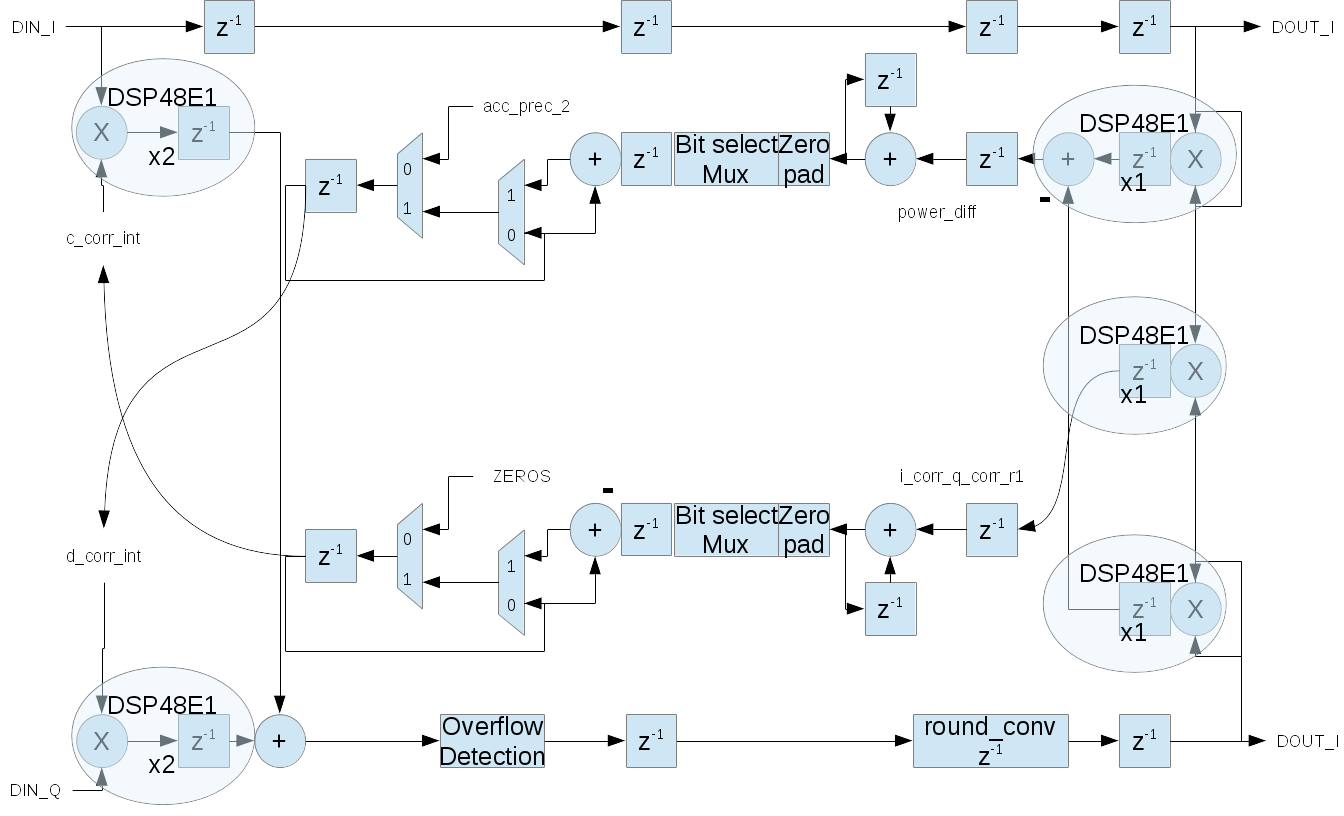
\includegraphics[scale=0.5]{iq_imbalance_block_diagram}\par\captionof{figure}{Block Diagram of VHDL, highlighting inferred Xilinx DSP48E1 primitives}\label{fig:iq_imbalance_block_diagram}}
\newpage

\section*{Worker Implementation Details}
\subsection*{\comp.hdl}
\begin{flushleft}
	The IQ Imbalance Fixer worker inputs complex signed samples and removes the spectral image caused by a quadrature gain imbalance between I and Q rails and also by a phase imbalance (not a perfect 90 degrees between sine and cosine) between the complex rails. The averaging time and the error loop gain of the worker are programmable, as is the ability to bypass the worker and to update/hold the calculated error correction values. For the HDL worker, a generic controls inclusion of a peak detection circuit applied to the worker's output samples.\medskip

	An \verb+ENABLE+ input is available to either enable (true) or bypass (false) the circuit. Note that bypass registers are not used. Instead, feedback error values are held constant at values that do not alter the Q rail. The \verb+UPDATE+ input, by default true, may be disabled to hold the loop errors to a constant value. Note that the \verb+ENABLE+ input takes priority over the \verb+UPDATE+ input.\medskip

	This implementation uses seven Xilinx DSP48e multipliers to process input data at the clock rate - i.e. this worker can handle a new input value every clock cycle. A peak detection circuit may be optionally included at build-time, which provides monitoring of the output amplitude, and may be used to influence the input gain. This worker will produce valid output four clock cycles after each valid input.\medskip

	The IQ Imbalance Fixer worker utilizes the OCPI \textit{iqstream\_protocol} for both input and output ports. The \textit{iqstream\_protocol} defines an interface of 16-bit complex signed samples. The \verb+DATA_WIDTH_p+ parameter may be used to reduce the worker's internal data width to less than 16-bits.
\end{flushleft}

\section*{Theory}
\begin{flushleft}
	A mathematical representation of a quadrature signal is given by the formula $cos(2\pi t/T)+jsin(2\pi t/T)$. If we let $\omega=2\pi t/T$, the equation of an imbalanced quadrature signal is $cos(\omega)+j\alpha sin(\omega+\beta)$, where $\alpha$ is the amplitude difference and $\beta$ is the phase difference between I/Q rails. If we take the imbalanced signal and mix it with another frequency, such as upconverting or downconverting the signal, we essentially multiply the input signal by the tone $cos(\omega0)+jsin(\omega0)$. The output signal then becomes a frequency-shifted version of the input signal given by $cos(\omega-\omega0)+j\alpha sin(\omega-\omega0+\beta)$. The result is a spectral image of the original signal at $-(\omega-\omega0)$. In the case of a non- zero linear combination of sine and cosine waves (which we have from a quadrature A/D, where the Q rail is simply a phase shift of $\pi/2$ of the I rail), we may use the trigonometric identity $\alpha sin(x+\beta) = Ccos(x) + Dsin(x)$, where C and D are constants and are the phase and amplitude errors applied to the I and Q input values, respectively. Thus the corrected output rails become I and $CI+DQ$.
\end{flushleft}

	\section*{Block Diagrams}
	\subsection*{Top level}
	\begin{center}
		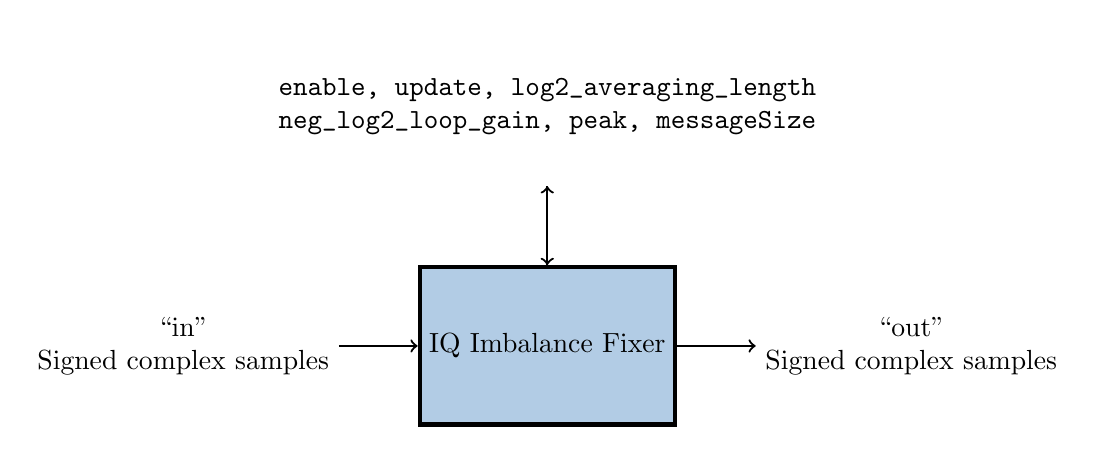
\begin{tikzpicture}[% List of styles applied to all, to override specify on a case-by-case
				every node/.style={
					align=center,  		% use this so that the "\\" for line break works
					minimum size=2cm	% creates space above and below text in rectangle
				},
				every edge/.style={draw,thick}
			]
			\node[rectangle,ultra thick,draw=black,fill=blue](R2){\Comp};
			\node[rectangle,draw=white,fill=white](R3)[left= of R2]{``in" \\ Signed complex samples};
			\node[rectangle,draw=white,fill=white](R4)[right= of R2]{``out" \\ Signed complex samples};
			\node[rectangle,draw=white,fill=white](R5)[above= of R2]{\verb+enable, update, log2_averaging_length+\\ \verb+neg_log2_loop_gain, peak, messageSize+};
			\path[->]
			(R3)edge []	node [] {} (R2)
			(R2)edge []	node [] {} (R4)
			(R2)edge []	node [] {} (R5)
			(R5)edge []	node [] {} (R2)
			;
		\end{tikzpicture}
	\end{center}

	\subsection*{State Machine}
	\begin{flushleft}
		Only one finite-state machine (FSM) is implemented by this worker. The FSM supports Zero-Length Messages.
	\end{flushleft}
	{\centering\captionsetup{type=figure}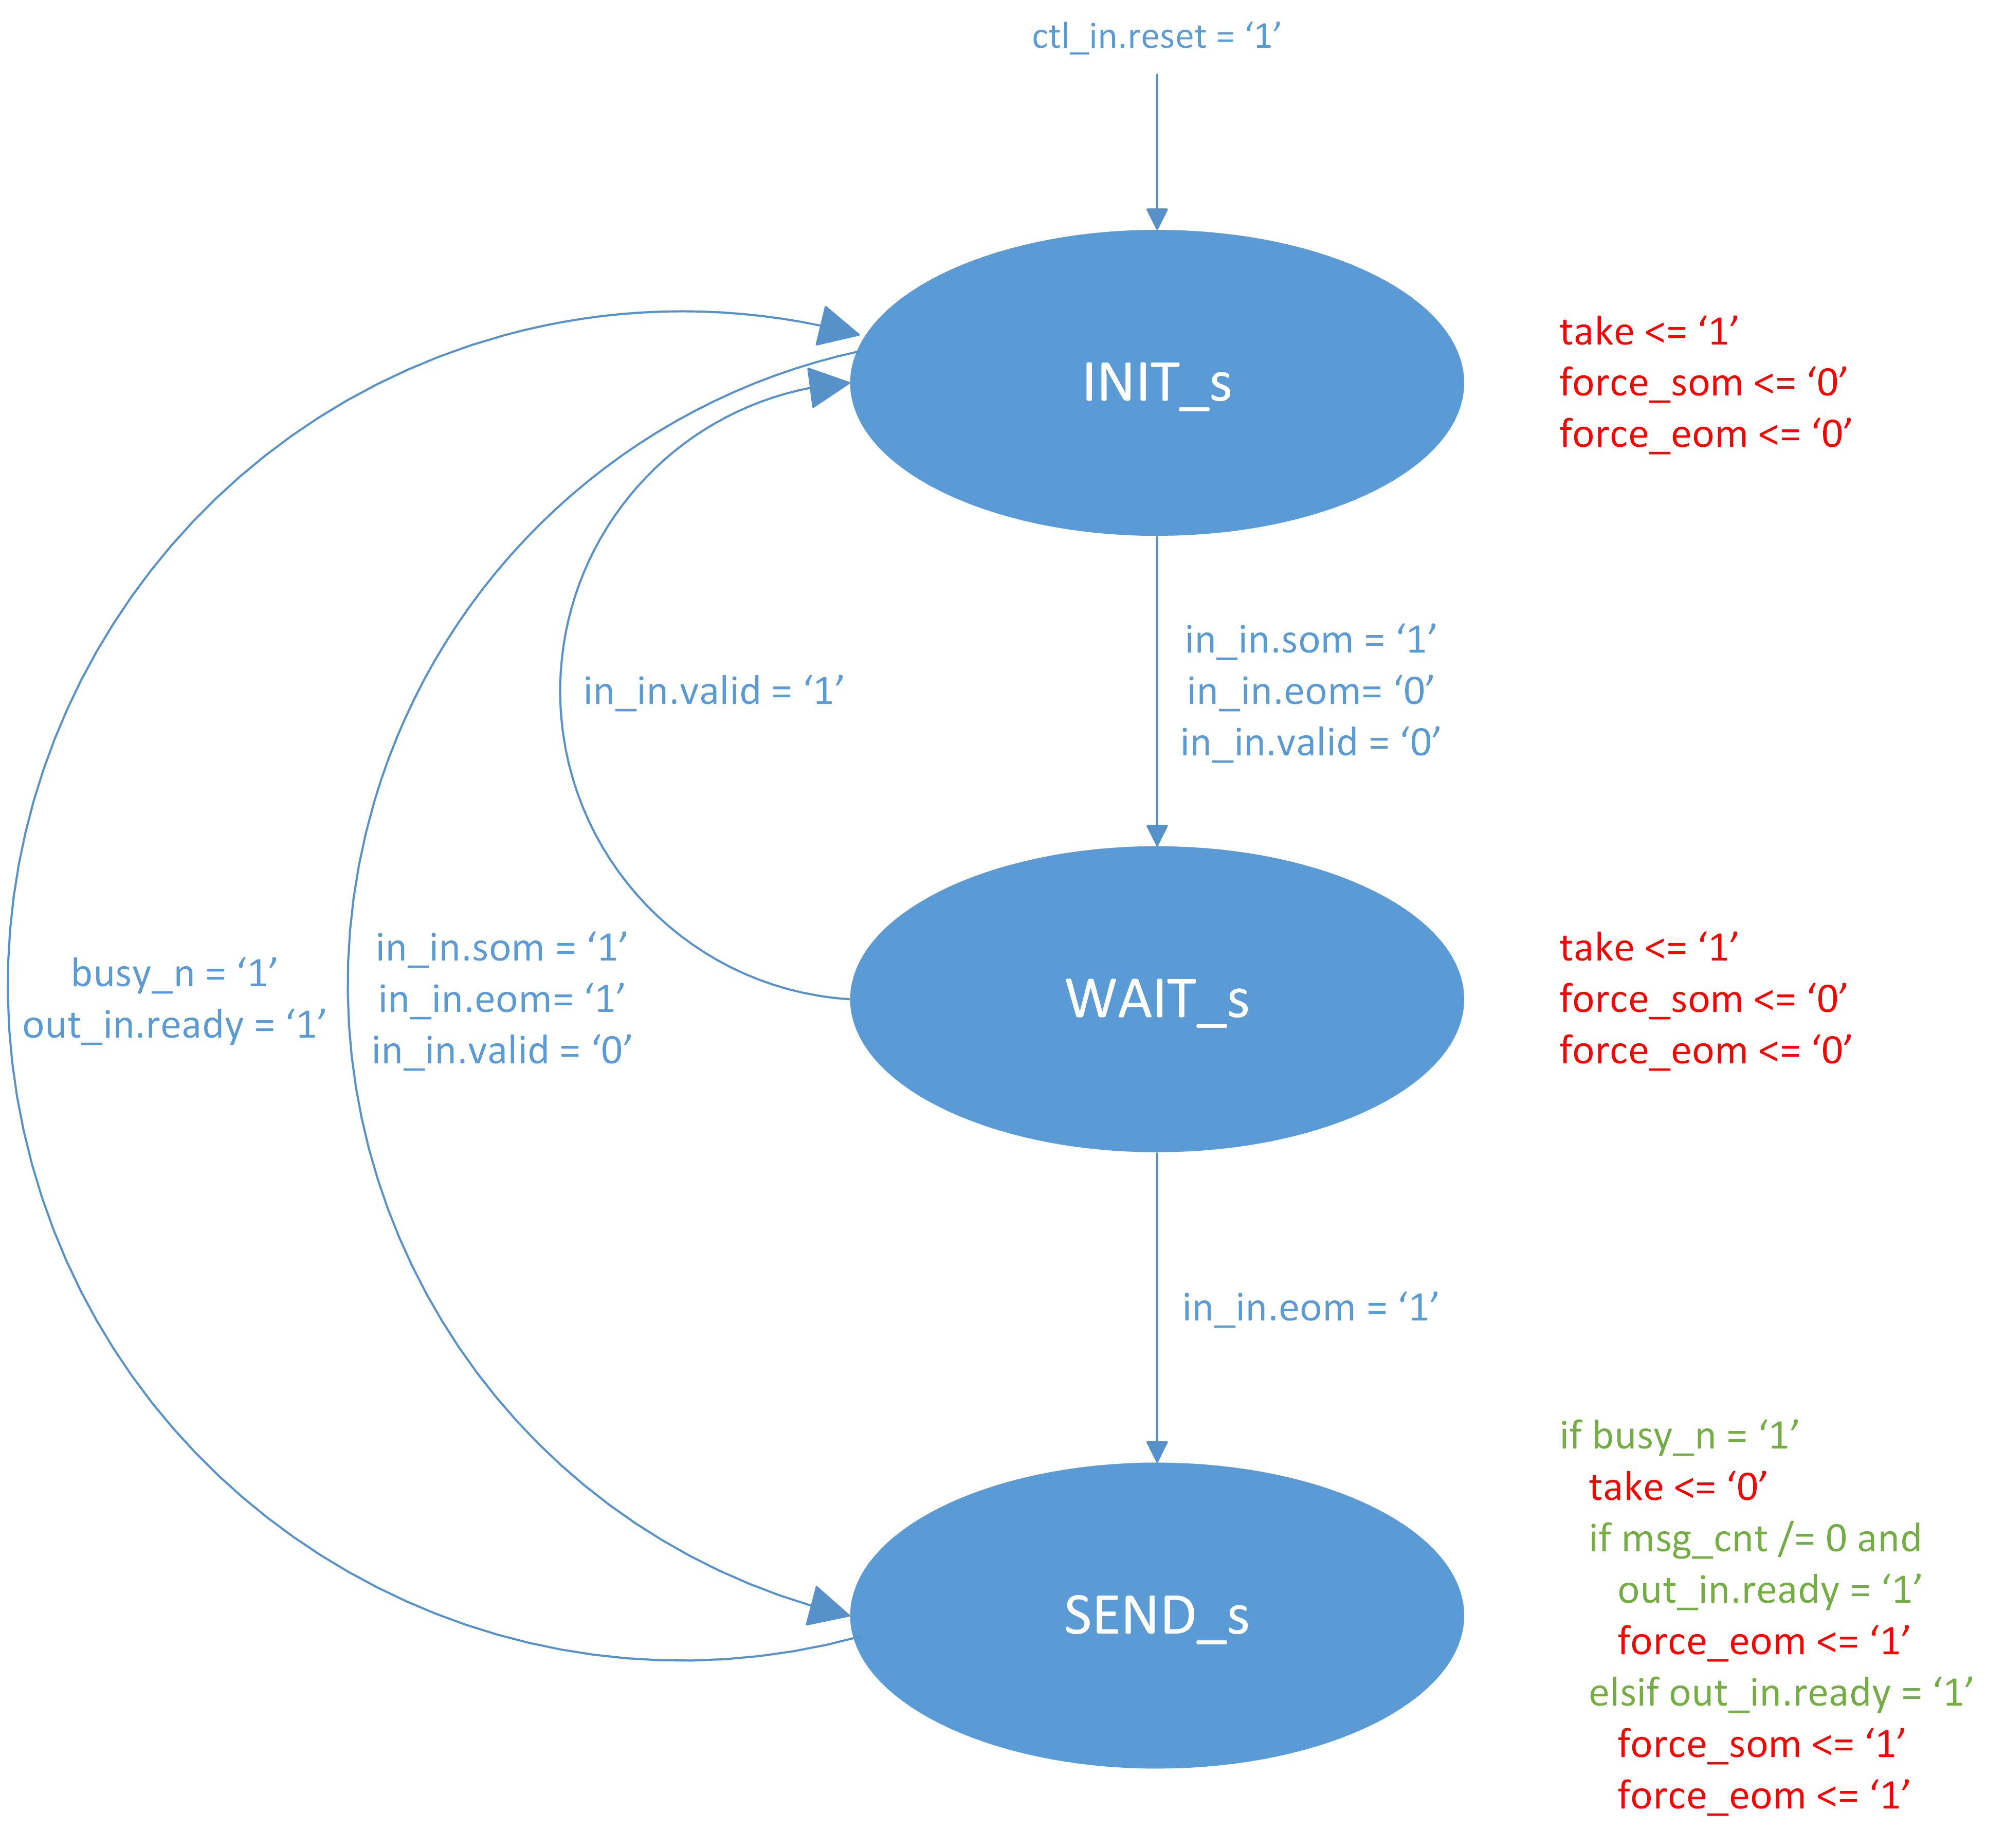
\includegraphics[scale=0.6]{zlm_fsm}\par\captionof{figure}{Zero-Length Message FSM}\label{fig:zlm_fsm}}
        \begin{flushleft}
                Note: In future releases this finite-state machine will be replaced with a register-delay based mechanism, currently exemplified in the dc offset filter
        \end{flushleft}

	\newpage

	\section*{Source Dependencies}
	\subsection*{\comp.hdl}
	\begin{itemize}
		\item ocpiassets/components/dsp\_comps/iq\_imbalance\_fixer/iq\_imbalance\_fixer.vhd
		\item ocpiassets/hdl/primitives/dsp\_prims/dsp\_prims\_pkg.vhd
		      \subitem ocpiassets/hdl/primitives/dsp\_prims/iq\_imbalance/src/iq\_imbalance\_corrector.vhd
		\item ocpiassets/hdl/primitives/util\_prims/util\_prims\_pkg.vhd
		      \subitem ocpiassets/hdl/primitives/util\_prims/pd/src/peakDetect.vhd
	\end{itemize}

	\begin{landscape}
		\section*{Component Spec Properties}
		\begin{scriptsize}
			\begin{tabular}{|p{3cm}|p{1.5cm}|c|c|c|c|c|p{7cm}|}
				\hline
				\rowcolor{blue}
				Name                         & Type   & SequenceLength & ArrayDimensions & Accessibility      & Valid Range & Default & Usage                                                                                                      \\
				\hline
				\verb+enable+                & Bool   & -              & -               & Writable, Readable & Standard    & true    & Enable/bypass control                                                                                      \\
				\hline
				\verb+update+                & Bool   & -              & -               & Writable, Readable & Standard    & true    & Update the calculated amplitude and phase errors, or hold a previously calculated value                    \\
				\hline
				\verb+log2_averaging_length+ & UChar  & -              & -               & Writable, Readable & 1-31        & 11      & Controls the update interval to be applied to the input, where $2^n+1$ samples define the averaging length \\
				\hline
				\verb+neg_log2_loop_gain+    & UChar  & -              & -               & Writable, Readable & 1-31        & 5       & Controls the loop gain, where the value is $2^{-n}$                                                        \\
				\hline
				\verb+messageSize+           & UShort & -              & -               & Writable, Readable & 8192        & 8192    & Number of bytes in output message                                                                          \\
				\hline
			\end{tabular}
		\end{scriptsize}

		\section*{Worker Properties}
		\subsection*{\comp.hdl}
		\begin{scriptsize}
			\begin{tabular}{|p{3cm}|p{2cm}|p{1cm}|c|c|c|c|c|p{5cm}|}
				\hline
				\rowcolor{blue}
				Type     & Name                  & Type  & SequenceLength & ArrayDimensions & Accessibility       & Valid Range & Default & Usage                                        \\
				\hline
				Property & \verb+DATA_WIDTH_p+   & ULong & -              & -               & Readable, Parameter & 1-16        & 16      & Worker internal non-sign-extended data width \\
				\hline
				Property & \verb+ACC_PREC_p+     & ULong & -              & -               & Readable, Parameter & 3-?         & 34      & Accumulator bit width                        \\
				\hline
				Property & \verb+PEAK_MONITOR_p+ & Bool  & -              & -               & Readable, Parameter & Standard    & true    &
				Include a peak detection circuit\\
				\hline
				Property & \verb+peak+           & Short & -              & -               & Volatile            & Standard    & 0       &
				Read-only amplitude which may be useful for gain control\\
				\hline
			\end{tabular}
		\end{scriptsize}

		\section*{Component Ports}
		\begin{scriptsize}
			\begin{tabular}{|M{2cm}|M{1.5cm}|M{4cm}|c|c|M{9cm}|}
				\hline
				\rowcolor{blue}
				Name & Producer & Protocol           & Optional & Advanced & Usage                  \\
				\hline
				in   & false    & iqstream\_protocol & false    & -        & Signed complex samples \\
				\hline
				out  & true     & iqstream\_protocol & false    & -        & Signed complex samples \\
				\hline
			\end{tabular}
		\end{scriptsize}
		\section*{Worker Interfaces}
		\subsection*{\comp.hdl}
		\begin{scriptsize}
			\begin{tabular}{|M{2cm}|M{1.5cm}|c|c|M{12cm}|}
				\hline
				\rowcolor{blue}
				Type            & Name & DataWidth & Advanced                & Usage                  \\
				\hline
				StreamInterface & in   & 32        & ZeroLengthMessages=true & Signed complex samples \\
				\hline
				StreamInterface & out  & 32        & ZeroLengthMessages=true & Signed complex samples \\
				\hline
			\end{tabular}
		\end{scriptsize}
	\end{landscape}

	\section*{Control Timing and Signals}
	\begin{flushleft}
		The IQ Imbalance Fixer worker uses the clock from the Control Plane and standard Control Plane signals.
	\end{flushleft}

	\section*{Performance and Resource Utilization}
	\subsubsection*{\comp.hdl}
	Table entries are a result of building the worker with the following parameter set:\
	\begin{itemize}
		\item \verb+DATA_WIDTH_p+=16
		\item \verb+ACC_PREC_p+=34
		\item \verb+PEAK_MONITOR_p+=true
	\end{itemize}
	\begin{scriptsize}

		\begin{tabular}{|c|c|c|c|c|c|}
			\hline
			\rowcolor{blue}
			Device                      & Registers & LUTs & Fmax        & Memory/Special Functions & Design Suite    \\
			\hline
			Stratix4 EP4SGX230K-C2-F40  & 950       & 1156 &            N/A & DSP 18x18 = 14           & Quartus Prime 15.1 \\
			\hline
			Virtex6 XC6VLX240T-1-FF1156 & 721       & 1477 & 163.827 MHz & DSP48E1 = 7              & ISE 14.7        \\
			\hline
			Zynq XC7Z020-1-CLG484       & 720       & 1089 & 125.109 MHz & DSP48E1 = 7              & Vivado 2017.1        \\
			\hline
			Zynq XC7Z020-1-CLG484       & 721       & 1506 & 161.577 MHz & DSP48E1 = 7              & ISE 14.7        \\
			\hline
		\end{tabular}
	\end{scriptsize}

	\section*{Test and Verification}
	\begin{flushleft}
	A single test case is implemented to validate the IQ Imbalance Fixer component. An input file is generated consisting of a waveform with tones at 5 Hz, 13 Hz, and 27 Hz, and creates a spectral image by both adding different gain to I and Q rails and also adding an additional 10 degrees of phase to the sine portion of the complex signal. The result is the addition of spectral image tones at -5 Hz, -13 Hz, and -27 Hz. The complex waveform is then scaled to fixed-point signed 16-bit integers, with a maximum amplitude of 31000 to avoid roll-over.\medskip

Time and frequency domain plots may be viewed in Figures \ref{fig:in_time_tone} and \ref{fig:in_freq_tone} below, respectively, where the time domain plot represents the first 128 complex samples in the file.
	\end{flushleft}

	\begin{figure}[ht]
		\centering
		\begin{minipage}{.5\textwidth}
			\centering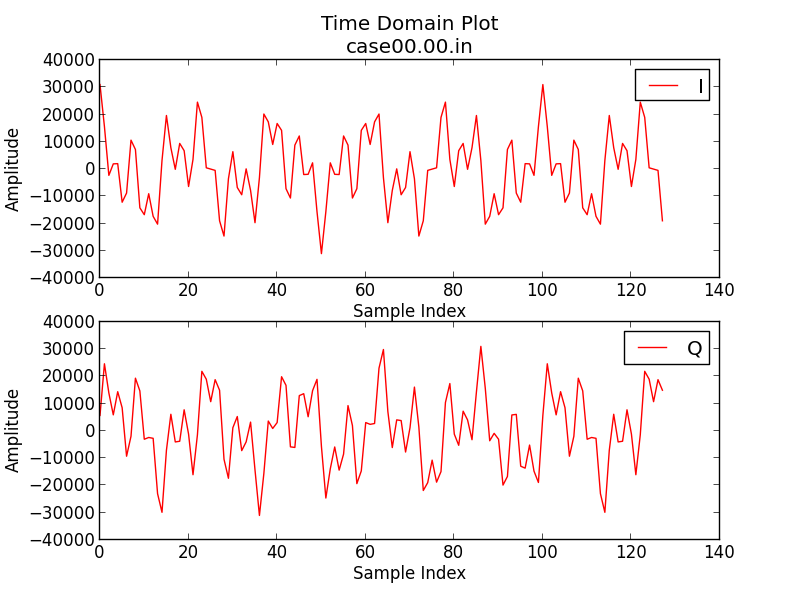
\includegraphics[width=1.0\linewidth]{input_time_tones}
			\captionof{figure}{Time Domain Tones with Spectral Image}
			\label{fig:in_time_tone}
		\end{minipage}%
		\begin{minipage}{.5\textwidth}
			\centering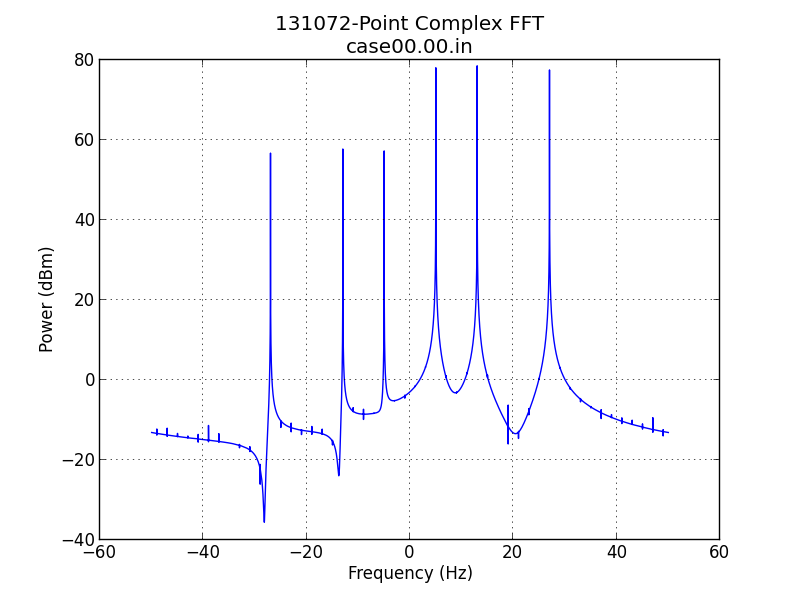
\includegraphics[width=1.0\linewidth]{input_freq_tones}
			\captionof{figure}{Frequency Domain Tones with Spectral Image}
			\label{fig:in_freq_tone}
		\end{minipage}
	\end{figure}

	\begin{flushleft}
	Verification of output data is performed only on the second half of the output, which represents the steady state of the component. The output is first checked that the data is not all zero, and is then checked for the expected length of 65,536 complex samples. Once these quick checks are made both the input and output data are translated to the frequency domain, where a FFT is performed, and then power measurements are taken at 5 Hz, 13 Hz, 27 Hz, -5 Hz, -13 Hz, and -27 Hz. The input and output power measurements are compared to validate that the IQ spectral image has been attenuated and that the other tones have not been attenuated. In addition, the FFT bin with the maximum power in the range of DC to +Fs/2 is compared to the maximum power bin in the range of -Fs/2 to DC to verify at least 65 dB of suppression has taken place with respect to the spectral image. Figures \ref{fig:out_time_tone} and \ref{fig:out_freq_tone} depict the filtered results of the three tone input, where the time domain plot represents the first 128 complex samples in the file.
	\end{flushleft}

	\begin{figure}[ht]
		\centering
		\begin{minipage}{.5\textwidth}
			\centering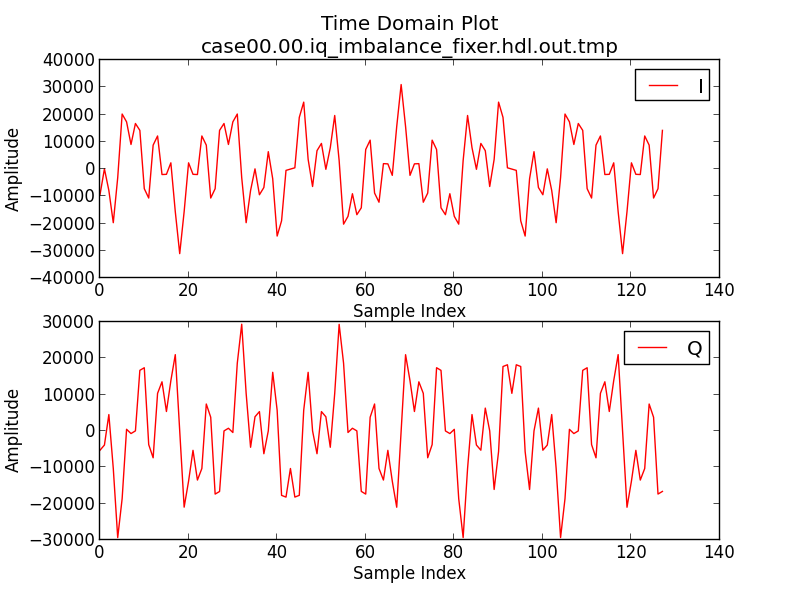
\includegraphics[width=1.0\linewidth]{output_time_tones}
			\captionof{figure}{Time Domain Tones with Spectral Image removed}
			\label{fig:out_time_tone}
		\end{minipage}%
		\begin{minipage}{.5\textwidth}
			\centering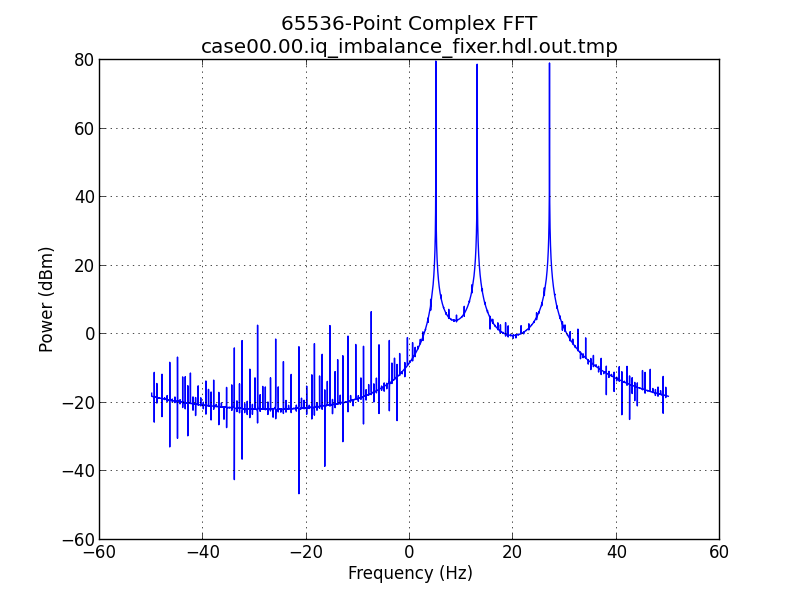
\includegraphics[width=1.0\linewidth]{output_freq_tones}
			\captionof{figure}{Frequency Domain Tones with Spectral Image removed}
			\label{fig:out_freq_tone}
		\end{minipage}
	\end{figure}
\end{document}
